\documentclass[11pt, letterpaper]{article}
\usepackage{../common}

\usepackage{url}
\usepackage{float}
\usepackage{amsfonts, amsmath, amsthm}
\usepackage{bm, tikz} % helpful packages
\usetikzlibrary{positioning}
\usepackage{listings}
\usepackage[shortlabels]{enumitem}
\usepackage{hyperref}
\usepackage{etoolbox}
\usepackage{mdframed}

\theoremstyle{definition}
\newtheorem{defn}{Definition}[section]
\theoremstyle{plain}
\usepackage[textsize=tiny]{todonotes}

% Some useful macros.
\newcommand{\R}{\mathbb{R}}
\newcommand{\C}{\mathbb{C}}
\newcommand{\E}{\mathbb{E}}
\newcommand{\var}{\text{Var}}
\newcommand{\cov}{\text{Cov}}
\newcommand{\p}{\partial}
\newcommand{\mb}{\bm}
\newcommand{\mba}{\bm{a}}
\newcommand{\mbb}{\bm{b}}
\newcommand{\mbx}{\bm{x}}
\newcommand{\mbxt}{\tilde{\bm{x}}}
\newcommand{\Sigmat}{\tilde{\Sigma}}
\newcommand{\mbz}{\bm{z}}
\newcommand{\mbw}{\bm{w}}
\newcommand{\eps}{\epsilon}
\newcommand{\Ut}{\tilde{U}}
\newcommand{\ind}{\perp \!\!\! \perp}
\newcommand{\angstrom}{\textup{\AA}}
\renewcommand{\v}[1]{\bm{#1}}

% Some settings: no indents, page numbers
\setlength\parindent{0pt}
\pagestyle{plain}

%%%%%%%%%%%%%%%%%%%%%%%%%%%%%%%%%%%%%%%%%%%
%% Solution environment
\usepackage{xcolor}
\newenvironment{solution}{
    \vspace{2mm}
    \color{blue}\noindent\textbf{Solution}:
}{}
%%%%%%%%%%%%%%%%%%%%%%%%%%%%%%%%%%%%%%%%%%%

\begin{document}

\begin{center}
{\LARGE CS 1810 Spring 2025 Midterm Review Session}\\
\end{center}

\section{Regression}

\subsection{Linear Regression and Loss Minimization}

In supervised learning, we have some data $\{ (\bm x^{(n)}, y^{(n)}) \}_{n=1}^N$ and seek to model/predict the output $y^{(n)}$ based on the inputs $\bm x^{(n)}$. We call the output our \textbf{target/response} variable and the inputs our \textbf{features/predictors}. In \textbf{linear regression} we form a prediction $\hat y$ based on a linear combination of the features as such:
\begin{align*}
    \hat y = \sum_{d=1}^D w_d x_d = \bm{w}^\top\bm{x}
\end{align*}
The weights $\bm w$ are our model \textbf{parameters}, and our task in linear regression is to learn these parameters. To solve for the optimal parameters, we need to define a \textbf{loss function} that depends on $\bm w$. The loss function captures how well our model fits the true data through outputting what is essentially an error metric. For ordinary least squares (OLS) regression, we use the \textbf{least squares} loss function:
\begin{align*}
    \mathcal{L}(\bm w; \bm{X}, \bm{y}) = \dfrac{1}{2}\sum_{n=1}^N\left(y^{(n)} - \bm{w}^\top\bm{x}^{(n)} \right)^2 = \frac{1}{2}||\bm y - \bm X \bm w||^2
\end{align*}
We want to find the value of $\bm w$ that minimizes the loss function. To compute this, we expand the loss function, compute its derivative, and solve for $\bm w$ which sets the derivative equal to 0:
\begin{align*}
    \mathcal{L}(\bm w; \bm{X}, \bm{y}) &= \frac{1}{2}\left(\bm{y}^\top\bm{y} - 2\bm{y}^\top\bm{X}\bm{w} + \bm{w}^\top\bm{X}^\top\bm{X}\bm{w} \right) \\
    \Longrightarrow \nabla_{\bm w}\mathcal{L} &= -\bm{X}^\top\bm{y} + \bm{X}^\top\bm{X}\bm{w} \\
    \Longrightarrow \bm{w}^*_{OLS} &= (\bm{X}^\top\bm{X})^{-1}\bm{X}^\top\bm{y}
\end{align*}
Note that we need $\bm{X}^\top\bm{X}$ to be invertible.

This procedure can be generalized to arbitrary parametric models and loss functions. The name of the game here is to fit the model parameters through solving for the values that minimize the loss function. Keep in mind that an analytical solution doesn't always exist.

\subsection{Probabilistic Regression and MLE}
In the previous subsection, we didn't make any assumptions on the joint distribution that our data were drawn from. We now suppose that our data is generated as such
\[y^{(n)} = \bm{w}^\top\bm{x}^{(n)} + \epsilon^{(n)}, \quad \epsilon^{(n)} \overset{\mathrm{iid}}{\sim} \mathcal{N}(0, \sigma^2),\]
The joint likelihood of the data is
\[p(\bm y | \bm X, \bm w, \sigma^2) = \prod_{n=1}^{N}\frac{\exp\left(-\frac{(y^{(n)} - \bm{w}^\top\bm{x}^{(n)})^2}{2\sigma^2}\right)}{\sigma\sqrt{2\pi}}\]
Hence, the log likelihood is
\[\log p(\bm y | \bm X, \bm w, \sigma^2) = -\frac{1}{2\sigma^2}\sum_{n=1}^{N} (y^{(n)}- \bm{w}^\top\bm{x}^{(n)})^2 - N\left(\log(\sigma) + \frac{1}{2}\log(2\pi)\right) \]
For simplicity, let's assume $\sigma^2$ is known so that we only care about estimating $\bm w$. To learn these parameters, we seek to maximize the log-likelihood. This is called \textbf{maximum likelihood estimation}. Observing the above equation, we see that clearly the solution to this problem is the same as the OLS estimator!

 \subsection{Basis Regression}
By default, linear regression only allows us to model linear relationships between the raw inputs $\bm x$ and the output $y$. However, we can apply \textbf{basis transformations} to our inputs in order to model non-linear relationships. Say the true data generating relationship is $f(x)=1+ x^2$: using the basis transformation $\phi(x) = [1 \ x \ x^2]^\top $ would let us perfectly model the function with $\bm w = [1 \ 0 \ 1]^\top$ while a linear regression would model the relationship very poorly.  In general, we use a basis function $\phi : \mathbb{R}^D \to \mathbb{R}^M$ to formulate a prediction as such:
\[ \hat y = \sum_{m = 1}^{M}w_m \phi_m(\bm{x}) =\bm{w}^\top{\phi}(\bm{x})\]
Observe that we just treat the transformed inputs in the same way that we treated the raw inputs in the simple linear regression from earlier. To merge the bias term, we can define $\phi_1(\bm{x})=1$. Some examples of basis functions include polynomial $\phi_m(x) = x^m$, Fourier $\phi_m(x) = \cos( m \pi x )$, and Gaussian $\phi_m(x) = \exp \{- \frac{(x - \mu_m)^2}{2s^2}\}$. 

\subsection{Nonparametric Regression}
A \textbf{nonparametric} regression method makes no assumptions about the structure underlying the data. \textbf{$k$-Nearest Neighbors} ($k$-NN) is one of these methods since for a fixed value of $k$ that you choose, there are no other parameters that the model learns. Here is a rundown of the $k$-NN Algorithm:
    \begin{enumerate}
        \item Let $\bm{x}^*$ be the point that we would like to make a prediction about. Let's find the $k$ nearest points $\{\bm{x}^{(1)}, \ldots, \bm{x}^{(k)}\}$ to $\bm{x}^*$, based on some predetermined distance function.
        \item Denote the true $y$ values of these $k$ points as $\{y^{(1)}, \ldots, y^{(k)} \}$.
        \item Output our prediction $\hat{y}^*$ for our point of interest $\bm{x}^*$:
        \[\hat{y}^* =  \frac{1}{k}\sum_{n=1}^{k}y^{(n)}\]
    \end{enumerate}

    \textbf{Kernel regression} is considered to be a smoother, more general extension of $k$-NN. In Kernel regression, we want to take a \emph{weighted average} of all the points in our training data when forming a prediction for an unknown point. Intuitively, we want to weigh points that are ``closer" to our unknown point of interest \emph{more heavily} than points that are ``farther" away. Define $K(\bm{x}^*, \bm{x})$ as our kernel function, which we will use to weigh each point. The kernel function $K(\bm{x}^*, \bm{x})$ should be \emph{larger} for a point $\bm{x}$ closer to our point of interest $\bm{x}^*$ than a point $\bm{x}$ farther away. Importantly, the value of $\bm{x}$ that results in the largest value of $K(\bm{x}^*, \bm{x})$ should be $\bm{x}^*$ itself: 
    \[\textnormal{arg}\max_{\bm{x}} K(\bm{x}^*, \bm{x}) = \bm{x}^{*}\]
    Here is a rundown of kernel regression:
    \begin{enumerate}
        \item Let $\{\bm{x}^{(1)}, \ldots, \bm{x}^{(N)}\}$ (and their corresponding $y$ values) be \emph{all} of the $N$ points comprising our training data set. \item Let $\bm{x^{*}}$ be our point of interest that we want to make a prediction for. We make our prediction as follows:
        \[\hat{y}^* = \frac{\sum_{n=1}^{N}K(\bm{x}^*, \bm{x}^{(n)}) y^{(n)}}{\sum_{n=1}^{N}K(\bm{x}^*, \bm{x}^{(n)})}\]
    \end{enumerate}
    The denominator term normalizes the sum of our weights to equal $1$. Compared to the $k$-NN algorithm, the kernel regression uses all the points in the dataset to predict rather than just the $k$ nearest. 

\subsection{Exercises}

\begin{mdframed}
    \begin{enumerate}
        \item Problem
        
        \begin{solution}
            Solution
        \end{solution}

        \item Problem
        
        \begin{solution}
            Solution
        \end{solution}
    \end{enumerate}
\end{mdframed}

\section{Classification}
\subsection{Perceptron and Gradient Descent}

 We now move on to \textbf{classification}.
\begin{enumerate}
    \item Goal: Given an input vector $\bm x$, assign it to one of $K$ discrete \textbf{classes} $C_k$. Examples of classes include star types or spam vs. regular emails.
    \item Strategy: Divide our input space into \emph{disjoint} (i.e., no overlap) \textbf{decision regions} whose boundaries are called \textbf{decision boundaries/surfaces}. Each decision region corresponds to being assigned to a certain class: there should be $K$ decision regions if we are working with $K$ discrete classes.
\end{enumerate}

In \textbf{binary linear classification}, we are working with two classes divided by a linear separator in our feature space. We will denote the two classes as $-1$ and $1$ (note that in other situations, we might use $0$ and $1$). \textbf{Perceptron} is a non-probabilistic binary linear classification algorithm that uses a \textbf{discriminant function} $h$ to assign a given observation to a specific class, based on $\bm x$. Perceptron uses the sign of the discriminant to predict as such:
\[\hat{y} = \text{sign}(h(\bm x; \bm w, w_0)) = \text{sign}(\bm{w}^\top\bm{x} + w_0),\]
where $\text{sign}(z) = 1$ if $z \geq 0$, and $\text{sign}(z) = -1$ if $z < 0$.  To fit the optimal weights, we must first define a loss function. By construction of $\hat y$, we note that $h(\bm{x}^{(n)};\bm{w},w_0) y^{(n)}$ is positive when $\hat{y}^{(n)} = y^{(n)}$ and negative when $\hat{y}^{(n)} \ne y^{(n)}$. Hence, we use the hinge loss / ReLU:
\begin{align*}
   \mathcal{L}(\bm{w}) &=  \sum_{n=1}^N \text{ReLU}(-h(\bm{x}^{(n)};\bm{w},w_0) y^{(n)})  \\
    &=  -\sum_{n: y^{(n)} \neq \hat{y}^{(n)}} (\bm{w}^\top\bm{x}^{(n)} + w_0) y^{(n)}
\end{align*}
We can't analytically solve for the minimizer of this loss, but we can use \textbf{gradient descent}. This is a type of numerical method which iteratively updates the weights $\bm{w}$ at each timestep $t$ based on gradient information from some subset of the data. The general form of gradient descent is 
\[\bm{w}^{(t+1)} = \bm{w}^{(t)} - \eta \nabla_{\bm w}\mathcal{L},\]
where $\eta$ is the learning rate (hyperparameter). Different forms of gradient descent use a different subset of the data to compute/approximate the gradient $\nabla_{\bm w}\mathcal{L}$. \textbf{Batch gradient descent} uses the entire dataset, \textbf{stochastic gradient descent} uses a randomly selected subset, and the perceptron algorithm only uses one observation. This means that perceptron updates its weights one data point at a time as such:
\[
    \bm{w}^{(t+1)} = \bm{w}^{(t)} - \eta \nabla_{\bm w}\mathcal{L}^{(n)} = \bm{w}^{(t)} + \eta y^{(n)}\bm{x}^{(n)},
\]
where $\mathcal{L}^{(n)}$ is the loss for data point $n$. 

\subsection{Logistic Regression}

Like with regression, we can also take a probabilistic view on classification. \textbf{Discriminative models} are one of two distinct types of probabilistic classification models. These models focus on modeling $p(y | \bm x)$. Here is a rundown of \textbf{logistic regression}, a discriminative model for binary classification:
\begin{enumerate}
    \item Rather than using $-1$ and $1$ for our two classes, we now use $0$ and $1$. 
    
    \item We use the following probabilistic model:
    \[p(y = 1 | \bm{x}, \bm w) = \sigma(\bm{w}^{T}\bm{x}), \quad p(y = 0 | \bm{x}, \bm w) = 1 - \sigma(\bm{w}^{T}\bm{x} ),\]
    where $\sigma$ is the \textbf{sigmoid function}:
    \[\sigma(z) = \frac{1}{1 + \exp(-z)}\]
    Note that the sigmoid function maps the real line to $(0, 1)$, corresponding to probabilities.

    \item We'll use maximum likelihood estimation to find the optimal weights $\bm{w}$. The joint likelihood of the data is
    \[p(\bm y | \bm X, \bm w) = \prod_{n=1}^{N} p(y^{(n)}|\bm x^{(n)}, \bm w)\]
    Hence, the log likelihood is 
    \[\log p(\bm y | \bm X, \bm w) = \sum_{n=1}^{N} \log p(y^{(n)}|\bm x^{(n)}, \bm w)\]
    We can use the \textit{power trick}, which gives us the following decomposition:
    \[p(y |\bm x, \bm w) = p(y =1|\bm x, \bm w)^y \cdot p(y =0|\bm x, \bm w)^{1-y}\]
    You can also recognize that this is just the PMF of a Bernoulli. Substituting, we have that the log-likelihood is
    \begin{align*}
        \log p(\bm y | \bm X, \bm w) &= \sum_{n=1}^{N} \log\left(p(y^{(n)} =1|\bm x^{(n)}, \bm w)^{y^{(n)}} \cdot p(y^{(n)} =0|\bm x^{(n)}, \bm w)^{1-y^{(n)}} \right) \\
            &= \sum_{n=1}^{N} \left(y^{(n)} \cdot \log p(y^{(n)} =1|\bm x^{(n)}, \bm w) +  (1-y^{(n)}) \cdot \log p(y^{(n)} =0|\bm x^{(n)}, \bm w)\right) \\
            &= \sum_{n=1}^{N} \left(y^{(n)} \cdot \log \sigma(\bm{w}^\top \bm x)+  (1-y^{(n)}) \cdot \log (1-\sigma(\bm{w}^\top \bm x))\right)
    \end{align*}
    Maximizing this log-likelihood is equivalent to minimizing the negative log-likelihood. Hence, we can treat $-\log p(\bm y | \bm X, \bm w)$ as our loss function, take the gradient with respect to $\bm w$ and find the weights that set the gradient equal to zero. There is no analytical solution, so we use gradient descent to solve for the optimal $\bm w$.
\end{enumerate} 
Recall that this formulation can be extended to multi-class classification through using the softmax function instead of the sigmoid function.


\subsection{Generative Models and Naive Bayes}

\textbf{Generative Models} are the other type of probabilistic classification model. These incorporate the complete data generation process into its model via the \emph{joint distribution} $p(\bm{x}, y)$ of the class $y$ and the input data point $\mathbf{x}$. Note that Bayes' Rule allows us to decompose the joint as such:
\[p(\bm{x}, y) = p(\bm{x}|y)p(y)\]
Hence, we can impose distributions for $p(y)$, the \textbf{class prior}, and $p(\bm{x}|y)$, the \textbf{class-conditional distribution} to specify a complete generative model. To form predictions, we pick the class $C_k$ that maximizes $p(y=C_k|\bm{x})$. Note that the definition of conditional probability tells us that 
\[p(y|\bm{x}) \propto p(\bm x, y) = p(\bm{x}|y)p(y),\]
so we have all the information we need to predict using our generative model.

\textbf{Naive Bayes} is one type of generative model for classification. The key property of this general model is the ``naive'' assumption that each feature $x_d$ is \textit{conditionally independent} given the class of the target. This can be mathematically formulated as such:
\[p(\bm x |y = C_k) =  \prod_{d=1}^D p(x_d|y=C_k)\]
We use Naive Bayes to limit the number of parameters needed to specify our model. If our features were dependent on each other, then we would need to explicitly model this dependence using additional parameters. Here we only need the class prior $p(y)$ and the conditional probabilities $p(x_d | y=C_k)$ to specify our generative model.
\subsection{Exercises}
\begin{mdframed}
    \begin{enumerate}
        \item In the softmax setting, why must $p(y=k\mid \mathbf{x})$ sum to 1 across all classes $k$? Explain in words how softmax generalizes logistic regression from the binary case to the multi-class case. Suggest a method to make decision boundaries nonlinear without changing the form of the softmax function.
        
        \begin{solution}
            The sum across all classes is necessarily 1 because the output of the softmax function is a probability distribution over all classes. Softmax is the multi-class analog of the sigmoid used in logistic regression since we have multiple exponentiated linear functions normalized by their sum. To make decision boundaries nonlinear, we can use basis functions to transform the input space before applying softmax.
        \end{solution}

        \item You are comparing two classifiers for a multi-class classification problem: Naive Bayes and logistic regression. Both achieve roughly the same training loss, but on the validation set Naive Bayes does much worse. Give a high-level reason why Naive Bayes might underperform when the "naive" conditional independence assumption is violated by the real data. In another scenario, your data is very sparse. Which classifier would you expect to perform better, and why?
        
        \begin{solution}
            Naive Bayes can underperform when features are strongly correlated since it models them as conditionally independent given the class. In the sparse data regime, Naive Bayes would likely perform better since it requires fewer parameters to estimate (note that parameter growth is linear in the number of features) and imposes stronger assumptions on the data. In particular, having fewer parameters to learn reduces the risk of overfitting compared to a more complex model.
        \end{solution}
    \end{enumerate}
\end{mdframed}


\section{Model Selection}
\subsection{Bias-Variance Decomposition}
For a given supervised learning task, we ultimately want to select a model that predicts well on unseen data. One thing we can do is examine the mean squared errors of several candidate models on a validation set. We can also reason about this more generally through analyzing the expected squared error $\mathbb{E}_{D, y|\bm x}[(y - f_D(\bm x))^2]$ of our trained model $f_D$. In particular, the \textbf{bias-variance decomposition} tells us that 
\[
    \mathbb{E}_{D, y|\bm x}[(y - f_D(\bm x))^2] = \mathbb{E}_{y|\bm x}[(y- \mathbb{E}_{y|\bm x}[y])^2]+ \left(\mathbb{E}_{y|\bm x}[y]-\mathbb{E}_D[f(\bm x)]\right)^2 + \mathbb{E}_D[(\mathbb{E}_D[f(\bm x)]-f_D(\bm x))^2]
\]
Using more condensed notation, this can also be expressed as 
\[\mathbb{E}_{D, y|\bm x}[(y - f_D(\bm x))^2] = \underbrace{\mathbb{E}_{y|\bm x}[(y- \overline{y})^2]}_{\text{Noise}} + \underbrace{\left(\overline{y}-\overline{f}(\bm x)\right)^2}_{\text{Bias}^2} + \underbrace{\mathbb{E}_D[(\overline{f}(\bm x)-f_D(\bm x))^2]}_{\text{Variance}}\]
Let's review how to interpret each of these three terms:
\begin{enumerate}
    \item \textbf{Noise}: This captures the inherent variability in the values that you'd get from repeatedly sampling $y \sim p(y | \bm x)$. 
    
    \item \textbf{Bias}: This captures how far off your average prediction (over all possible training datasets) of $y$ from $\bm x$ is from the average value of $y$ given $\bm x$.
    
    \item \textbf{Variance}: This captures how much your prediction of $y$ from $\bm x$ varies depending on the dataset $D$ that your model $f_D$ was trained on.
\end{enumerate}
We usually describe the tradeoff between bias and variance through the concepts of \textbf{overfitting} and \textbf{underfitting}. An overfit model tends to have low bias but high variance. An example would be a degree 1000 polynomial regressor. A common symptom of an overfit model is a low train MSE but a high test MSE.  On the other hand, an underfit model tends to have a high bias but low variance. An extreme example is using a constant model such as $f_D = 0$. As far as the train and test MSEs, we'd likely see these both be similar but high.

\subsection{Improving Models: Ensemble Methods and Regularization}
Given the bias-variance decomposition, we can naturally think of improving our model through either reducing bias or reducing variance. \textbf{Ensembling} is a general approach that takes advantage of multiple models to obtain better predictive accuracy than with a single model alone. \\

In \textbf{bagging}, we resample ``new'' datasets from the training set (this is called \textit{bootstrapping}), fit a strong learner (relatively flexible/complex model) on these datasets, and combine the predictions from the strong learners. This method works by reducing the variance of these strong learners, which already have a relatively low bias. An example is the random forest, which is an average of predictions from decision trees! \\

In \textbf{boosting}, we train a series of weak learners (relatively simple models) sequentially. After training the $i^{th}$ model on a sample of the training set, we train the $(i+1)^{th}$ model on a new sample based on the performance of the $i^{th}$ model. The idea is that the examples classified incorrectly in the previous step receive higher weights in the new sample, encouraging the new model to focus on those examples. We then combine the predictions of these models through a weighted average. This method works by reducing the bias of the weak learners, which already have low variance. The Adaboost algorithm is an example of boosting. \\

Another commonly used approach for improving models is \textbf{regularization}, which focuses on reducing variance. We will discuss this in the context of linear regression, but it can be generalized to other model classes too. Taking degree $d$ polynomial regression as an example, we note that if we set $d$ too high, we get overfitting. Regularization addresses this problem through adding a \textbf{penalty term} $R(\bm w)$ to the loss function. Specifically, we have something of the form:
\[\mathcal{L}_{reg}(\bm w; \bm X, \bm y) = ||\bm y - \bm X \bm w||^2 + \lambda R(\bm w)\]
We can then solve for the optimal $\bm w$ that minimizes this loss function. With regards to specifying the penalty terms, we've discussed two main ones:
\begin{enumerate}
    \item \textbf{LASSO}: $R(\bm w) = ||\bm w||_1 = \sum_{d=1}^{D}|w_d|$. There is no closed-form solution, so numerical methods like cyclic coordinate descent are used. LASSO is unique in that it performs feature selection, i.e. it sets certain $w_d$ equal to 0.
    \item \textbf{Ridge}: $R(\bm w) = ||\bm w||^2 = \sum_{d=1}^{D}w_d^2$. There is a closed form:
    \[\bm w_{ridge} = (\bm{X}^\top\bm{X} + \lambda \bm I)^{-1}\bm{X}^\top\bm{y}\]
\end{enumerate}

\subsection{Bayesian Model Selection}
When using parametric methods, we sometimes may have some pre-existing belief about the parameters that we capture through a \textbf{prior} $p(\bm \theta)$. Then in the model selection process, we essentially hope to pick a model that fits the data well and aligns with our prior beliefs. Here is a review on the main components of Bayesian model selection:
\begin{itemize}
	\item We use Bayes' Rule to combine our prior with the likelihood, forming a \textbf{posterior}: 
    \[p(\bm \theta | \bm X, \bm y) \propto p(\bm y|\bm X, \bm \theta) p(\bm \theta)\]
    If we want a point estimate, we can solve for the value of $\bm \theta$ that maximizes this posterior.
	\item The \textbf{posterior predictive} for new data: 
    \[p(y^*|x^*, \bm X, \bm y) = \int p(y^*|x^*, \bm \theta) p(\bm \theta | \bm X, \bm y) d\bm \theta\]
	This tells us how to predict the label of a new data point according to the posterior over models obtained by updating the prior with the observed data.
	\item The \textbf{marginal likelihood} of data: 
    \[p(\bm y|\bm X) = \int p(\bm y|\bm X, \bm \theta) p(\bm \theta) d\bm \theta\]
	This tells us how likely the data is, marginalizing over all possible models $\bm \theta$. The marginal likelihood allows us to compare different priors or even different model classes in terms of how well they fit the data---this is precisely model selection!
\end{itemize}
To summarize, in Bayesian Regression, we encode our assumptions within the prior distribution $p(\bm \theta)$, which is updated in the posterior distribution $p(\theta|\bm X,\bm y)$. The posterior functions as our updated beliefs after seeing our data $\bm X,\bm y$, along with the most likely model for that data. The posterior predictive enables us to leverage the data we have seen to create predictions across all potential models (hence, the name). Finally, the marginal likelihood helps describe the likelihood of the data (producing $\bm y$ given $\bm X$ and the model $\bm \theta$) and can be interpreted in model selection as selecting the model that yields the highest likelihood of producing the data distribution (most likely to explain the result).

\subsection{Exercises}

\begin{mdframed}
    \begin{enumerate}
        \item You train a regression model and notice that MSE is nearly zero on training set but high on validation set, with large fluctuations in predictions for slightly different training subsets. What does this suggest about bias and variance? Propose two strategies to address the problem without gathering more data, and discuss how the strategies might help lower validation MSE.
        
        \begin{solution}
            Low training loss and high validation loss in the model suggest low bias and high variance, which we call overfitting. Strategies include adding regularization, decreasing model complexity, and using ensemble methods such as bagging. Variance is reduced and we generalize better since we are enforcing smoother or simpler functions, or averaging over multiple models.
        \end{solution}

        \item To mitigate overfitting in your above model, you use regularization. You are debating whether to add an $\ell_1$ or $\ell_2$ penalty to the weights. Conceptually, how do the learned weights of these two regularization methods differ, and if you suspect that only a few of the features used are actually relevant, which one would you use and how can you choose the regularization strength?
        
        \begin{solution}
            The two methods are lasso and ridge. The former can drive some weights to exactly zero while the latter generally shrinks all weights toward zero. If you suspect that only a few features are relevant, you should use lasso. You can choose the regularization strength through cross-validation where a larger $\lambda$ enforces more shrinkage. Note that variance decreases, but bias may increase.
        \end{solution}

        \item Consider the following settings for choosing hyperparameters for a model: a single 80/20 split between training and validation data, a 5-fold cross-validation, and a leave-one-out cross-validation. Conceptually, why might the second setting be preferred over the first, and what are some advantages and disadvantages of the third setting?
        
        \begin{solution}
            The second setting is preferred over the first because it reduces variance by averaging over multiple splits. In addition, leave-one-out cross-validation has the advantage of using almost all datapoints for each training fold which reduces bias since there is more training data, but it can be computationally expensive and have high variance for the test folds.
        \end{solution}

    \end{enumerate}
\end{mdframed}

\section{Neural Networks}

\subsection{Feedforward Networks: Motivation and Setup}

\textbf{Neural networks} are a parametric model class that are ubiquitous in modern machine learning. They are widely used because of their ability to learn an adaptive basis, parameterized by weights. Neural networks are very popular because of just how adaptive these bases can be. Namely, we have several \textbf{universal function approximation} theorems which essentially state that various neural network architectures can approximate \textit{any} function when taken to be large enough. 

\begin{center}
    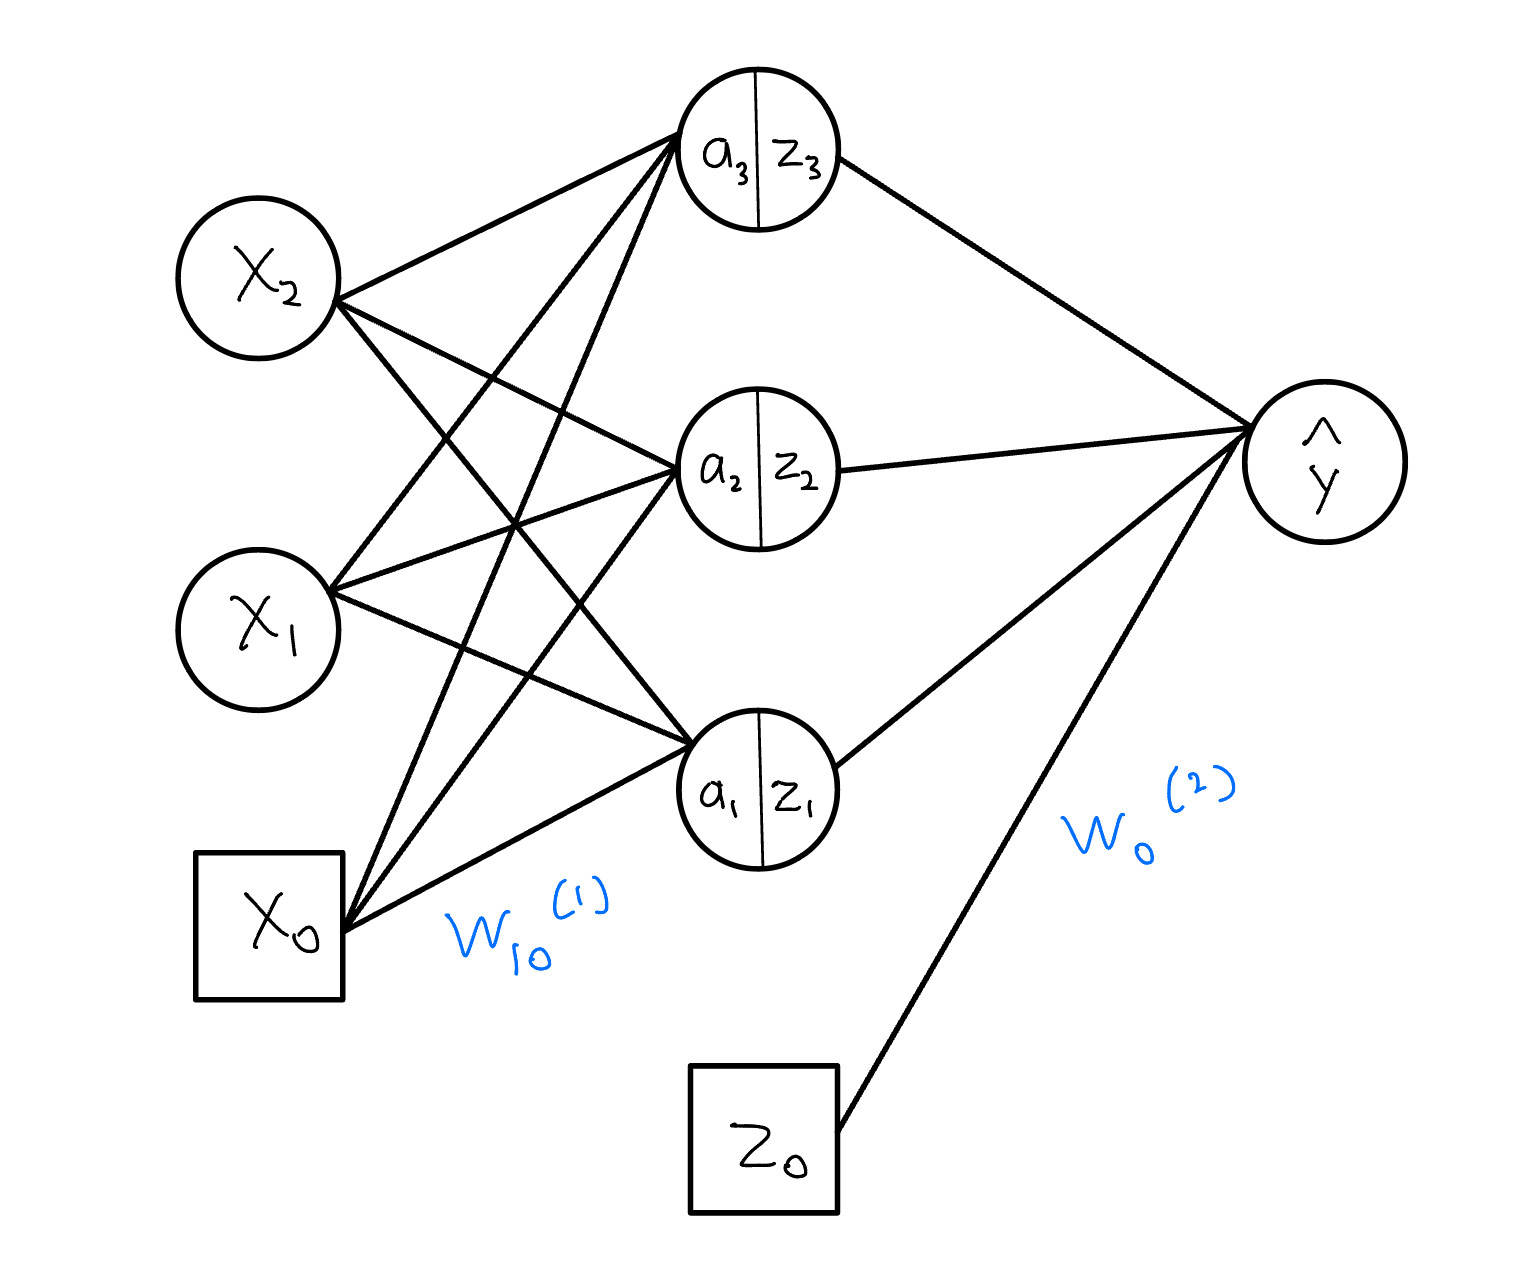
\includegraphics[scale=0.2]{img/nn_example.jpg}
\end{center}

Neural networks are essentially a series of connected \textbf{layers}, which are sets of \textbf{nodes}. The input layer consists of a node for each feature, while the output layer has as many dimensions as the target has. Any intermediate layers in between are called \textbf{hidden layers}. Finally, nodes are connected to each other by \textbf{connections}, which are parameterized by the model weights. A \textbf{feedforward network} is a type of NN in which information only ever flows along the direction of input to output. Mathematically, we can formulate the predictions from a simple NN with one hidden layer as such:
\[
\hat y = \bm w^{(2)}\bm z, \quad \bm z = h\left(\bm a\right), \quad \bm a = \bm{W}^{(1)}\bm x
\]
We call $\bm a$ the activation and $h$ the \textbf{activation function}, which we let be some nonlinear function. Some common activation functions are ReLU, tanh, and sigmoid. This nonlinearity within the neural network is precisely what allows them to be so flexible. 

\subsection{Neural Network Training}
To train neural networks, we use the framework of loss minimization via gradient descent. Thus, the main challenge is to compute the gradient of the loss with respect to all the weights. The overall process of training a neural network is called \textbf{backpropagation}. Let's consider the example of training the 3-layer feedforward network from above. Suppose we have the squared error loss function \(\mathcal{L}\) and we want to learn the weight \(w_{1, 0}^{(1)}\). To perform gradient descent, we need to compute \(\frac{\partial \mathcal{L}}{\partial w_{1, 0}^{(1)}}\). Considering the gradient for data point \(n\), we can use the chain rule as such:
\begin{align*}
\frac{\partial \mathcal{L}^{(n)}}{\partial w_{1, 0}^{(1)}} &=  \frac{\partial \mathcal{L}^{(n)}}{\partial \hat{y}^{(n)}} \cdot \frac{\partial \hat{y}^{(n)}}{\partial z_1} \cdot \frac{\partial z_1}{\partial a_1} \cdot \frac{\partial a_1}{\partial w_{1, 0}^{(1)}} \\
    &=  (y^{(n)} - \hat{y}^{(n)}) \cdot w^{(2)}_1 \cdot h'\left(a_1\right) \cdot x_0^{(n)}
\end{align*}
Note that we need $x_0^{(n)}$, $a_1$, and $\hat{y}^{(n)}$ in order to evaluate these gradients. These are all inputs/outputs along the network. The process by which an input \(\bm{x}^{(n)}\) is fed through the network to produce a prediction $\hat{y}^{(n)}$ is called the \textbf{forward pass}, and we store all the intermediate values along the way. We leverage this chain rule decomposition of the partial derivatives to efficiently compute them via one \textbf{backward pass} through the network. Working with a more general feedforward network, we can decompose each partial derivative as such:
\[\frac{\partial \mathcal{L}^{(n)}}{\partial w_{j, m}^{(l)}} =  \frac{\partial \mathcal{L}^{(n)}}{\partial a_j^{(l)}} \cdot \frac{\partial a_j^{(l)}}{\partial w_{j, m}^{(l)}} = \left(\sum_{j'=1}^{J_{l+1}} \frac{\partial \mathcal{L}^{(n)}}{\partial a_{j'}^{(l+1)}} \cdot \frac{\partial a_{j'}^{(l+1)}}{\partial a_{j}^{(l)}}\right) \cdot z_{m}^{(l-1)},\]
where we assume that layer $l$ of the network has $J_l$ nodes. Note that $\frac{\partial \mathcal{L}^{(n)}}{\partial a_j^{(l)}}$ can be written in terms of the derivatives with respect to the activations from the subsequent layer. This shows that we can compute each \textit{error} $\frac{\partial \mathcal{L}^{(n)}}{\partial a_j^{(l)}}$ starting from the end of the network and going to the start (this is why we call it the backward pass), reusing the precomputed partial derivatives from later in the network to compute the partial derivatives from the layer immediately before. Combined with the input/output values $z_m^{(l-1)}$ that we got from the forward pass, we now have our complete backpropagation method. As seen here, the key idea behind backpropagation is to reuse intermediate results (activations, inputs to each layer, the final output, and the errors) to efficiently compute the gradient of the loss with respect to the network weights.

\subsection{Exercises}

\begin{mdframed}
    \begin{enumerate}
        \item Problem
        
        \begin{solution}
            Solution
        \end{solution}

        \item Problem
        
        \begin{solution}
            Solution
        \end{solution}
    \end{enumerate}
\end{mdframed}

\section{Support Vector Machines}

\subsection{Hard Margin Formulation}
\textbf{Support vector machines} (SVM's) are classification models that use a linear model of the decision boundary to perform classifications. The idea behind them is that, for all the linear hyperplanes that exist, we want one that will create the largest distance with the training data. At a high level, we define the margin as the minimum distance between a point and our boundary. Larger margins tend to improve generalization error.

Now we'll put this into math. To find a mathematical formula for the margin, we consider a hyperplane of the form
\[\bm{w}^\top \bm x + w_0 = 0.\]
Furthermore, we can compute the signed distance $r$ between any point $\bm{x}^*$ and the hyperplane as such:
\[r = \frac{\bm{w}^\top\bm{x}^*+w_0}{||\bm{w}||}\]
Then, note that for a correctly classified data point $n$, we have $y^{(n)}=+1$ when this distance is positive and $y^{(n)}=-1$ when it is negative. So, we can obtain a positive distance for both kinds of examples by multiplying the above expression by $y^{(n)}$ (which will not change the magnitude since $\|y^{(n)}\| =  1$). Then, we can define the \textbf{margin }of the dataset as the minimum such distance over all of our $\bm{x}^{(n)}$ in our dataset:
\[\min_{n} \frac{y^{(n)}(\bm{w}^\top\bm{x}^{(n)} + w_0)}{||\bm{w}||}\]
Now to find the optimal $\bm{w}$, \textbf{hard margin} SVM's solve the following problem:
\[\argmax_{\boldw,w_0} \frac{1}{||\boldw||} \min_n y^{(n)}(\boldw^\top\boldx^{(n)}+w_0)\]
Now assume the data are completely linearly separable. This implies that the margin of the dataset is positive. Observing that $\bm{w}$ and $w_0$ are invariant to changes of scale, it is without loss of generality to impose
$\min_{n} y^{(n)}(\boldw^\top\boldx^{(n)} + w_0) \ge 1$. This lets
us write the optimization problem as:
\[\argmin_{\boldw, w_0} \frac{1}{2}||\boldw||^2 \quad \text{ s.t. }\forall n\text{ }
y^{(n)}(\boldw^\top\boldx^{(n)}+w_0) \geq 1\]

\subsection{Soft Margin Formulation}
Recall that towards the end of the hard margin derivation, we imposed the assumption that the dataset is linearly separable. However, this is not always true, and even if the data are linearly separable, it may not be ideal to find a separating hyperplane. In optimizing generalization error, there is a
tradeoff between the size of the margin and the number of mistakes on the training data. For the \textbf{soft margin} formulation, we introduce a \textbf{slack variable} $\xi^{(n)}
\geq 0$ for each $n$ to relax the constraints on each example.
%
$$
\xi^{(n)} \begin{cases}
      =0 & \text{if correctly classified and not inside margin region} \\
      \in (0,1] & \text{if correctly classified but inside margin
        region}\\
      >1 & \text{if incorrectly classified}
   \end{cases}
$$

\noindent We can now rewrite
the training problem
for a soft margin formulation to be
%
$$
\argmin_{\boldw, w_0, \bm \xi} \frac{1}{2}{||\boldw||^2} + C\sum_{n=1}^N \xi^{(n)} $$
$$\text{ s.t. }\forall n \text{ } y^{(n)}(\boldw^\top\boldx^{(n)}+w_0) \geq 1 - \xi^{(n)}$$
$$ \xi^{(n)} \geq 0$$


\noindent We add a regularization parameter $C$, that controls how much we
penalize violating the hard margin constraints.
A large $C$ penalizes these violations and thus
``respects'' the data closely and has small regularization.  A small
$C$ does not penalize the sum of slack variables as heavily, relaxing
the constraint. This is increasing the regularization.

\subsection{Dual Form of SVM Training}
Let's return to our training problem, specifically from the hard margin formulation. You will not need to know the details of the derivation for the exam, but just be aware that Lagrange multipliers and duality are used to derive the following solution for the optimal $\bm w$:
\[\bm{w}^* = \sum_{n=1}^N (\alpha^*)^{(n)}y^{(n)}\bm{x}^{(n)}\]
The optimal $w_0$ can be solved for by using the equation
\[y^{(n)}((\bm{w}^*)^\top\bm{x}^{(n)} + w_0) = 1\]
for any point $n$ on the margin boundary. Note that $\bm{\alpha}^*$ is solved for via quadratic programming methods beyond the scope of the class. Substituting $\bm{w}^*$ into the discriminant, we see that the SVM classifies a new example $\bm{x}$ through computing
\[\sum_{n=1}^N (\alpha^\star)^{(n)} \,y^{(n)} (\bm{x}^{(n)})^\top \bm{x}+w_0^*\]
Based on this, we classify the example as $+1$ if this discriminant value is $>0$, and $-1$ otherwise. We note that the only training points which matter for prediction are those with $(\alpha^*)^{(n)} > 0$. Naturally, we define these points to be the \textbf{support vectors}. Under the hard margin formulation, the support vectors lie right along the margin boundaries. Under the soft margin formulation, the support vectors may also lie within the margin region or even be misclassified.

\subsection{Kernel Trick}

Additionally, the dual has the very nice property that
if we use a basis function to map $\bm{x}$ to a higher dimensional space, this only comes in through the \textbf{kernel function}. The training problem is the same as explained earlier, except we replace
$(\bm{x}^{(n)})^\top \bm{x}^{(n')}$ with
\[K(\bm{x}^{(n)},\bm{x}^{(n')}) = \phi(\bm{x}^{(n)})^\top\phi(\bm{x}^{(n')})\]
Similarly, we classify a new example $\bm{x}$
based on the value of discriminant
\[\sum_{n=1}^N{\alpha^\star}^{(n)} \,y^{(n)}K(\bm{x}^{(n)},\bm{x}) +w_0^*.\]
The reason that this is interesting
is because we can directly compute the dot product
$\phi(\bm{x}^{(n)})^\top\phi(\bm{x})$
{\em without projecting to the higher-dimensional space!}
This is known as the \textbf{kernel trick}. As long as $K()$ is a valid kernel, the dual training problem can be solved without actually computing $\phi$. Note that we can use this trick specifically because the dual gives us an equation for $\bm{w}^*$ in terms of $\phi(\bm{x}^{(n)})^T\phi(\bm{x})$.



\subsection{Exercises}

\begin{mdframed}
    \begin{enumerate}
        \item Problem
        
        \begin{solution}
            Solution
        \end{solution}

        \item Problem
        
        \begin{solution}
            Solution
        \end{solution}
    \end{enumerate}
\end{mdframed}

\end{document}
